\chapter{Estado de la Cuestión}
\label{cap:estadoDeLaCuestion}


En este capítulo revisaremos los aspectos necesarios para la comprensión de los modelos que se exponen en los capítulos que siguen. La Sección \ref{sec:cuestInmuno} brinda unas nociones básicas sobre inmunología, en las que se trata brevemente el estudio de los mecanismos y agentes del sistema inmune necesarios para la respuesta ante una infección, destacando el papel de las células T. Esta sección constituye una parte fundamental del trabajo, pues los modelos que se presentan a continuación deben ser mirados y entendidos a través del problema inmunológico que se intenta explicar. Por su parte, la Sección \ref{sec:coop} habla sobre los modelos matemáticos en el campo de la biología y, más concretamente, sobre algunos de los que han intentado dar explicación al problema de decisión entre división o apoptosis de las células T durante una infección aguda. El desarrollo detallado del modelo de nuestro estudio puede verse en el Capítulo \ref{cap:descripcionTrabajo}.


\section{Cuestiones básicas de inmunología}
\label{sec:cuestInmuno}

Antes de comenzar es conveniente introducir una serie de definiciones y explicaciones básicas referentes al sistema inmune y a los procesos que este lleva a cabo. De esta manera, los conceptos y modelos que se expondrán más adelante serán entendidos en su contexto y sin ningún impedimento terminológico. Recordemos que, este trabajo se centra en el estudio de un modelo matemático que representa un aspecto concreto de la respuesta inmune. Es por ello que una noción, básica, como la que aquí se expone, sobre el sistema inmune es necesaria para su comprensión y posterior análisis.

En la Sección \ref{cap:introduccion} de Introducción ya decíamos que el sistema inmune funciona de manera colectiva, a pesar de las decisiones individuales que toman sus células. Este sistema está compuesto por diversos agentes de distinto tipo que trabajan de forma coordinada para dar una respuesta eficaz y proporcional al ataque recibido. Este último adjetivo es muy importante: necesitamos que la actuación de nuestro sistema inmune no sea insuficiente, lo que podría acarrear alguna inmunodeficiencia, ni tampoco excesiva, que es lo que ocurre, por ejemplo, con las alergias: el sistema inmune reacciona de manera exagerada a ciertos \textit{antígenos} que son, en la mayoría de casos, inofensivos. Otro de los requisitos que debe tener un buen sistema inmune es la capacidad para discriminar a quién hay que atacar y a quien no, evitando que las células del propio organismo sean blanco de su acción. Esto último es lo que sucede en el caso de las enfermedades autoinmunes, que pueden llegar a ser trastornos muy graves.

Describiremos brevemente a continuación los mecanismos de los que dispone el sistema inmune y cómo los utiliza. Haremos un recorrido desde lo más básico, comenzando por el \textit{sistema inmmune innato}, hasta conceptos más avanzados referentes al \textit{sistema inmune adaptativo}. Dedicaremos buena parte de esta sección a entender qué son las células T y cual es su papel en el desarrollo de una respuesta ante una infección aguda. Como veremos, este tipo de células inmunes juega un papel primordial y, además, serán las grandes protagonistas de este trabajo de fin de grado \citep{JTB}.  

\subsection{El sistema inmune innato}

Comencemos por lo más simple: las barreras físicas. La piel y la mucosa de nuestro sistema respiratorio, digestivo y reproductivo intentan que virus, bacterias, hongos o parásitos no entren en nuestro organismo. Es la primera defensa que tenemos y es bastante efectiva en muchos casos pero, ¿qué pasa si estos agentes logran atravesar esta barrera?

Aquí entra en juego lo que se denomina \textit{sistema inmune innato} que, desde el punto de vista evolutivo, es el más antiguo de los sistemas inmunes de los seres vivos. De hecho, muchos mecanismos de este sistema inmune innato aparecieron hace más de 500 millones de años \citep{theHowItWorks}. A pesar de que dispone de mecanismos mucho más sencillos que el \textit{adaptativo}, el papel que tiene es fundamental, pues permite dar una primera respuesta rápida ante una infección. 

Entre las armas de las que dispone encontramos proteínas, fagocitos y células NK (\textit{Natural Killer}), que son un tipo de linfocito producido en la médula ósea y que se distribuye por la piel, el intestino, el hígado, los pulmones y el útero, entre otros tejidos \citep{celulasNK}. Pero centrémonos en uno de sus componentes más relevantes: los \textit{macrófagos}. Su nombre compuesto por dos palabras griegas: \textit{macro}, que significa grande y \textit{fago}, que significa comer, lo dice todo. En efecto, los \textit{macrófagos} son células que se comen invasores mediante un proceso llamado \textit{fagocitosis}, que ilustra la Figura \ref{fig:macrofago}. El mecanismo es muy similar al utilizado por una ameba. Los \textit{macrófagos} rodean a una partícula sólida con su membrana, formando pequeños ``brazos'' conocidos como \textit{pseudópodos}. Una vez que el \textit{macrófago} tiene en un interior a la bacteria, la degrada en una vesícula llamada \textit{lisosoma}. Esta contiene sustancias que podrían degradar hasta el propio \textit{macrófago} si salieran de esta vesícula. 


\begin{figure}[t]
	\centering
	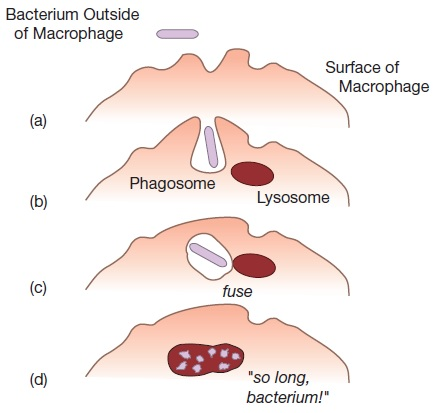
\includegraphics[width=0.5\textwidth]{1_macrofago}
	\caption{Fagocitosis.}
	\label{fig:macrofago}
\end{figure}


Durante la batalla con las bacterias, los \textit{macrófagos} producen y secretan unas proteínas llamadas \textit{citoquinas}, que facilitan la comunicación entre células del sistema inmune y que cobrarán un papel muy relevante en los capítulos que siguen.
Podríamos decir que los \textit{macrófagos} hacen el papel de centinelas, que cuando ven al enemigo mandan señales (\textit{citoquinas}) para reclutar a más defensores. A continuación, veremos otros tipos de células, en este caso referentes al \textit{sistema inmune adaptativo}.

\subsection{El sistema inmune adaptativo}


El nombre es bastante descriptivo y es que gracias a este sistema somos capaces de adaptar nuestras defensas a nuevos invasores. Pero no fue hasta la década de  1790 cuando tuvimos constancia de esta habilidad adaptativa. Por aquel entonces Edward Jenner, conocido como \textit{el padre de la inmunología}\footnote{\url{https://historia.nationalgeographic.com.es/a/edward-jenner-probablemente-cientifico-que-mas-vidas-ha-salvado-historia_14242}}, comenzó a vacunar a la población inglesa contra la viruela, que hasta entonces era una enfermedad temible. Lo que Jenner observó es que los ganaderos que se dedicaban a ordeñar vacas y que contraían el virus de la viruela bovina (\textit{cowpox}, en inglés) raramente contraían la viruela. Así que Jenner decidió llevar a cabo un experimento, poniendo en práctica el método conocido como \textit{variolización}\footnote{Este proceso consistía en inocular material infectado a una persona sana y fue introducido en Londres en 1721 por  Lady Montagu, esposa del embajador inglés en Turquía.} que aprendió en el hospital de San Jorge de Londres: para ello, guardó pus de uno de los ganaderos con viruela bovina y lo usó para inocular a un niño sano, James Phillips. El resultado fue una fiebre leve que desapareció a los pocos días, después Phillips fue reinoculado con pus proveniente de una persona con viruela, pero no contrajo la enfermedad. De esta manera, Jenner demostró que el sistema inmune humano podía proporcionar armas para protegernos de un intruso que no había visto antes, ¡había inventado la vacuna!. Es importante observar que la vacuna contra la viruela solo protegía contra esta enfermedad o algunas causadas por virus similares, como en el caso de la viruela bovina. Es decir, el sistema inmune adaptativo se adapta para defendernos de invasores \textit{específicos}. 

Veamos ahora en qué consiste la acción del sistema adaptativo. Para ello necesitamos hacer uso de los conceptos de \textit{antígeno} y \textit{anticuerpo}. Los \textit{anticuerpos} son proteínas específicas que el cuerpo humano es capaz de producir y que pueden adherirse a otras sustancias, externas o internas, llamadas \textit{antígenos}. La misión principal de los \textit{anticuerpos} es identificar a los \textit{antígenos} generados por un agente \textit{patógeno}, marcándolos así para su eliminación. Las encargadas de la producción de \textit{anticuerpos} son las células B. Estas son un tipo de linfocito blanco producido en la médula que, gracias a su receptor de membrana, son capaces de identificar a los \textit{antígenos}. Cuando las células B nacen no están especializadas en la fabricación de un \textit{anticuerpo} concreto, una vez que maduran, su ADN se recombina especializando así a la célula. Una vez que la célula B se encuentra con su \textit{antígeno} desencadenante, ésta produce muchas células grandes conocidas como \textit{células plasmáticas}. Cada \textit{célula plasmática} es esencialmente una fábrica para producir \textit{anticuerpos}. %Siempre que el \textit{anticuerpo} y el \textit{antígeno} se corresponden, el \textit{anticuerpo} marca el \textit{antígeno} para su destrucción. %Sin embargo, los linfocitos B no pueden penetrar en las células, de manera que el trabajo de atacar estas células diana se deja a los linfocitos T. 

Es decir, gracias a la presencia de \textit{anticuerpos}, otras células, como los ya conocidos \textit{macrófagos} son capaces de identificar a los elementos que hay que destruir cuando aún se encuentran en el medio extracelular como muestra la Figura \ref{fig:macrofago_anticuerpo}. Pero... ¿qué ocurre cuando un virus ya ha entrado en una célula de nuestro cuerpo? Los \textit{anticuerpos} no pueden alcanzarlo y el virus puede dedicarse a replicarse cuanto quiera. En este momento llega el turno de las protagonistas de este trabajo, las células T. 



\begin{figure}[t]
	\centering
	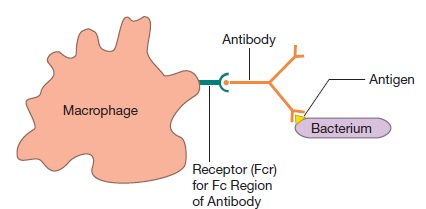
\includegraphics[width=0.6\textwidth]{2_macrofago_anticuerpo}
	\caption{Macrófago reconociendo una bacteria gracias a la acción \textit{anticuerpo-antígeno}.}
	\label{fig:macrofago_anticuerpo}
\end{figure}


\subsubsection{Las células T}
\label{Tcell}

Al igual que las células B, las células T se producen en la médula y ambas son muy similares en  cuanto a su apariencia, de hecho, con un microscopio ordinario, un inmunólogo no sería capaz de diferenciarlas \citep{theHowItWorks}. La superficie de las células T también consta de unas moléculas que permiten la interacción con los \textit{antígenos} llamados receptores (TCR, \textit{T Cell Receptors}). Estos receptores permiten a estas células obtener información de su entorno y tomar decisiones en base a esa información. Por ejemplo, cuando los receptores de una célula T enlazan con un \textit{antígeno} compatible, las células proliferan para dar lugar a otras con la misma especificidad, es decir, que enlacen con el mismo \textit{antígeno}. Esta decisión de reproducción, que discutiremos con más detalle en los capítulos que siguen, es específica y lenta, tarda alrededor de una semana en completarse \citep{theHowItWorks}, lo que contrasta con la respuesta rápida que nos ofrecía el \textit{sistema inmune innato}.

Hemos visto algunas de las similitudes que tienen las células B y T. Veamos algunas de sus diferencias: las células T maduran en el timo, de ahí la T de su nombre, mientras que las B maduran en la médula ósea. Además, las células B producen \textit{anticuerpos} que pueden reconocer cualquier molécula orgánica, las células T, por su parte, están especializadas en el reconocimiento de un \textit{antígeno} específico y sus receptores permanecen siempre adheridos a la membrana celular y no pueden ser expulsados en forma de \textit{anticuerpo} como en el caso de las células B. Pero, quizá, su diferencia más importante sea que las células T no pueden reconocer al \textit{antígeno} ``por sí mismas'', necesitan que otra célula se lo presente \citep{theHowItWorks}. Las células que se encargan de ello se conocen como \textit{células presentadoras de antígeno}\footnote{Son macrófagos, células dendríticas, células B, entre otras.}. Las proteínas del microorganismo causante de la infección, una vez fagocitadas, son fragmentadas (formando los conocidos \textit{antígenos}) y transportadas hasta la superficie celular, donde quedan unidas a una estructura llamada \textit{complejo mayor de histocompatibilidad} (MHC) que se encuentra en la membrana de las \textit{células presentadoras de antígeno}. Gracias a su TCR las células T pueden reconocer aquellas células que han sido infectadas, puesto que el TCR y el MHC-péptido\footnote{Estructura formada por el MHC y el \textit{antígeno}.} encajan, la Figura \ref{fig:antigen_presentation} ilustra este proceso. Esta unión, si es perfecta, dura varias horas y se conoce como \textit{sinapsis inmunológica} \citep{fernandez2012mecanica}.



Hay distintos tipos de células T atendiendo al papel que desempeñan, los tres más importantes son: 
\begin{itemize}
	\item \textit{Killer o Cytotoxic T-Cells}: su misión es la de reconocer las células que han sido infectadas y, tras este proceso de reconocimiento, las inducen al suicidio. De esta manera muere el virus pero también la célula que había sido infectada por él. Constituyen una de las armas más potentes del sistema inmune.
	
	\item \textit{Helper T-Cells}: se encargan de regular la respuesta inmune. Una de sus tareas principales es secretar \textit{citoquinas} para controlar que la respuesta inmune sea proporcional y las células T no reaccionen de manera descontrolada.
	
	\item \textit{Regulatory T-Cells}: estas mantienen la tolerancia a \textit{antígenos} propios, previniendo la aparición de enfermedades autoinmunes.
\end{itemize}



\begin{figure}[t]
	\centering
	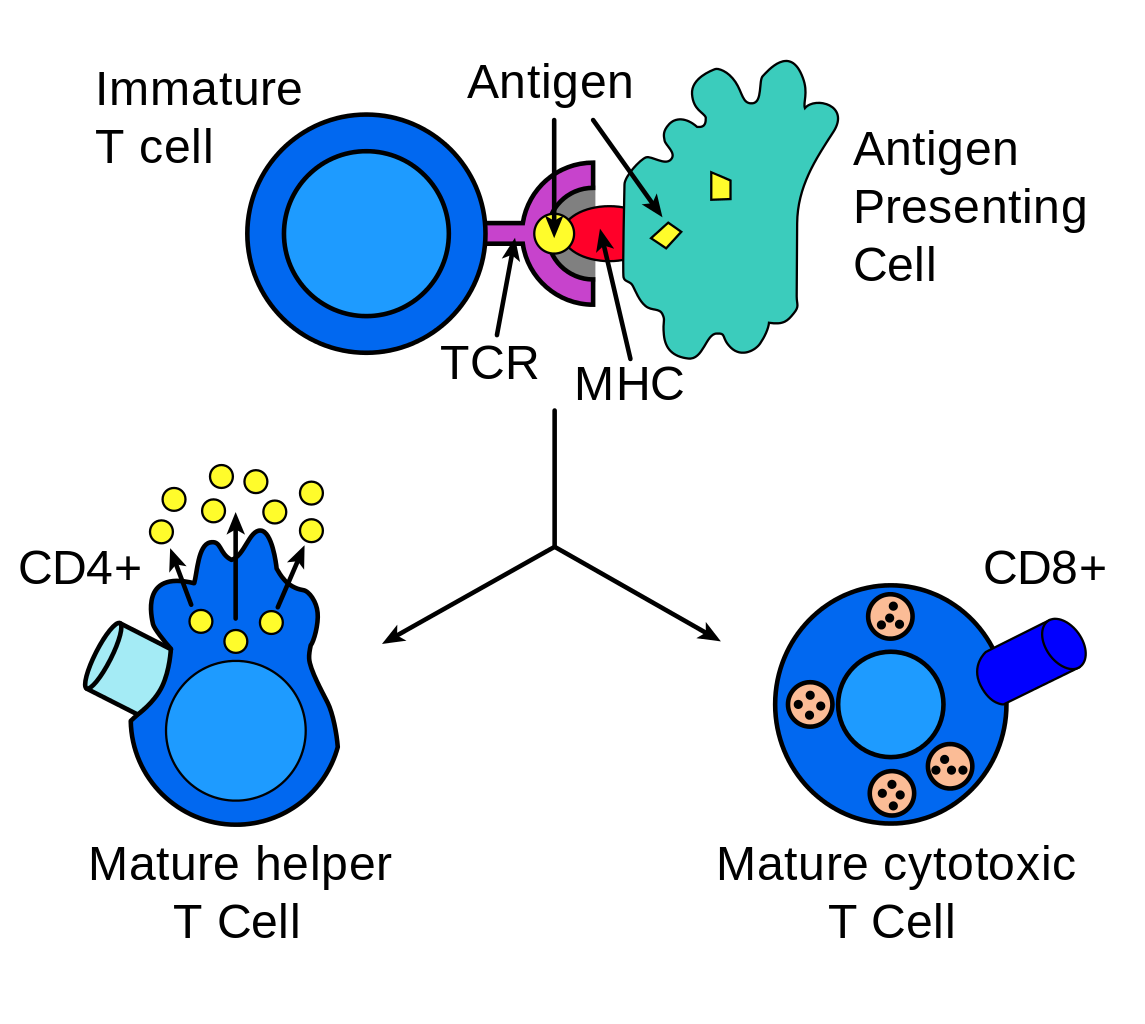
\includegraphics[width=0.6\textwidth]{Imagenes/EstadoDeLaCuestion/Antigen_presentation}
	\caption{Proceso de activación de una célula T.}
	\label{fig:antigen_presentation}
\end{figure}


Cuando las células T salen del timo se encuentran desactivadas, en un estado \textit{naïve} y se dedican a circular por los órganos linfoides secundarios, cuyo máximos representantes son los nodos linfáticos. Allí pueden encontrarse con \textit{células presentadoras de antígeno} provenientes del foco de una infección. Si las células T reconocen al \textit{antígeno} como extraño por medio de la \textit{sinapsis inmune}, se activan, convirtiéndose así en células efectoras, capaces de secretar \textit{citoquinas} o de ir a la zona afectada a combatir la infección activamente. Una vez que las células han sido activadas, estas comienzan a proliferar masivamente, incrementando la población de células T activadas hasta en un factor de $10^6$ veces, en pocos días, las células pueden pasar por unos 15-20 ciclos de reproducción \citep{JTB}. Este proceso se conoce como \textit{expansión clonal}. Una vez que las células \textit{helper} han sido activadas pueden quedarse en los gánglios linfáticos, activando a otras células inmunitarias, o migrar al tejido infectado para secretar \textit{citoquinas} y propiciar un ambiente adecuado para controlar la infección. Por su parte, las células \textit{killer} abandonan los gánglios linfáticos para identificar aquellas células infectadas en el organismo. Cuando el \textit{patógeno} ha sido vencido, la mayoría de células T mueren, restaurando así los niveles de población iniciales. Este proceso se conoce como \textit{contracción clonal}. Sin embargo, es de gran utilidad conservar alguna de estas células experimentadas para poder reaccionar con rapidez en caso de que el mismo invasor vuelva a aparecer. Lo que hace nuestro sistema inmune es mantener un pequeño porcentaje de la población  ($5-10\%$) como células de memoria \citep{JTB}. Se llaman así porque guardan información del \textit{antígeno} contra el que combatieron, son más fáciles de activar y nuestro cuerpo puede así generar una respuesta inmune más rápidamente.

A lo largo de este trabajo nos centraremos en el proceso de decisión entre división o suicidio celular de una célula T durante la respuesta inmune. En la sección y los capítulos que siguen veremos cómo se ha abordado este problema desde el punto de vista matemático y las conclusiones que su estudio ha permitido obtener. 


\section{Cooperación entre dos ciencias: Matemáticas y Biología}
\label{sec:coop}

En esta sección trataremos brevemente la interacción entre dos ciencias muy distintas: las matemáticas y la biología, y daremos algunos ejemplos de colaboraciones y modelos matemáticos creados para reproducir e investigar distintos procesos biológicos. Nos centraremos en aquellos referidos a las células T, sobre todo al caso que nos ocupa: la dinámica de población de las mismas durante la respuesta inmune.

Después de haber seguido un desarrollo independiente durante siglos, las matemáticas y la biología  han comenzado a interaccionar activamente durante los últimos años.
%
%A pesar de que las matemáticas han influido en investigaciones biológicas muy importantes como los trabajos de Gregor Mendel en genética y los de Theodor Boveri en la naturaleza de los cromosomas (\cite{mathsModInmu}, \cite{esteban2003mendel}), las colaboraciones matemáticas-biología no han sido muy frecuentes.Causa que puede ser justificada por el evidente contraste académico que tienen ambas y que veremos un poco más detalladamente en la sección siguiente. 
De hecho, los modelos matemáticos pueden llegar a ser una potente herramienta en el área de la biología. Como se puede leer en \cite{Gunawardena2014}, un modelo matemático es una máquina lógica que convierte hipótesis en conclusiones. Si el modelo es correcto y las hipótesis son ciertas entonces debemos, por lógica, creer sus conclusiones. Esta garantía lógica permite al matemático que desarrolla el modelo navegar con confianza lejos de las hipótesis y, probablemente, más lejos del lugar al que la mera intuición permite llegar. Sin embargo, no debemos confundirnos, los modelos no dan respuestas seguras. Esas respuestas son siempre consecuencia lógica de las hipótesis. En palabras de James Black\footnote{Biografía de este famoso farmacólogo: \url{https://www.britannica.com/biography/James-Black}}, los modelos matemáticos son descripciones precisas de nuestro patético pensamiento (<<\textit{accurate descriptions of our pathetic thinking}>>).

Así pues, los modelos matemáticos son herramientas en las que un biólogo se puede apoyar, pero estos modelos deben tener ciertas características para poder considerarse de utilidad por la comunidad de biólogos. A continuación se presentan las guías que sugiere \cite{Gunawardena2014} para elaborar un buen modelo matemático:

\begin{enumerate}
	\item \textit{Formula una pregunta}. En ocasiones los modelos matemáticos no son diseñados para el avance del conocimiento de la biología, solo responden a investigaciones matemáticas que se basan, aparentemente, en problemas biológicos. Como ya se ha comentado en alguna ocasión, los modelos deben centrarse en aportar información que el biólogo desconocía. Intentar responder con un modelo a una pregunta puede ser clave a la hora de desarrollarlo con criterio, para que pueda ser juzgado por profesionales fuera del ámbito matemático. 
	
	\item \textit{Hazlo simple}. Incluir todos los procesos bioquímicos puede tranquilizar a los biólogos pero no hará que el modelo sea mejor, de hecho se convertirá en un modelo repleto de parámetros, poco flexible, difícil de estudiar y simular. Es mejor tener hipótesis simples y claras, intentando buscar una abstracción del problema.
	
	\item \textit{Si el modelo no puede ser refutado, entonces no está diciendo nada interesante}. No es suficiente con que el modelo reproduzca hechos observados. En muchas ocasiones el ajustar demasiado el modelo provoca que lo seleccionemos para que se ajuste a lo que queremos explicar dejando un modelo poco flexible, que apenas aporta nuevo conocimiento.
\end{enumerate}

Podemos distinguir dos tipos de estrategia en cuanto a los modelos se refiere: Modelado hacia adelante (\textit{forward modeling}) o inverso (\textit{reverse modeling}). El modelado inverso empieza con los datos experimentales, construye correlaciones entre ellos y les da estructura con un modelo matemático. Por su parte, el modelado hacia adelante empieza desde lo conocido, o sospechado, expresado en la forma de un modelo, a partir del cual se hacen predicciones. 

El modelado inverso se ha utilizado con el fin de analizar grandes volúmenes de datos genómicos y postgenómicos y, a veces, se equipara erróneamente con la biología de sistemas. Ocasionalmente ha sugerido nuevas ideas conceptuales, pero se ha utilizado con mayor frecuencia para sugerir nuevos componentes o interacciones moleculares, que luego han sido confirmados por enfoques biológicos convencionales. Los modelos en sí mismos han tenido menos importancia para comprender el comportamiento del sistema que como contexto matemático en el que la inferencia estadística se vuelve factible. En contraste, las mayores aportaciones a nuestra comprensión del comportamiento de problemas biológicos como la homeostasis o la retroalimentación, han surgido del modelado hacia adelante. Puesto que los modelos actuales (cimentados en ecuaciones diferenciales o teoría de procesos estocásticos, por ejemplo) derivan, normalmente, de fenómenos y conocimiento conocidos. El primer beneficio que se obtiene de esto es que fuerzan al modelo a establecer unas hipótesis claras \citep{mathsModInmu}. Esto no implica que el modelado inverso no sea interesante. Hay muchas situaciones, especialmente cuando se tratan datos clínicos, donde la estructura de los datos se desconoce o es muy compleja, y las estrategias del modelado inverso cobran sentido \citep{Gunawardena2014}. 

El descubrimiento del microscopio a finales del siglo XVII provocó una revolución en la biología al revelar mundos invisibles y anteriormente desconocidos. Las matemáticas pueden ser interpretadas en la actualidad como un microscopio más general, ya que, pueden revelar mundos invisibles en todo tipo de datos, no solo ópticos. Por ejemplo, la tomografía computarizada puede revelar una sección transversal de una cabeza humana a partir de la densidad de los rayos X sin necesidad de abrir la cabeza. Charles Darwin tenía razón cuando escribió que las personas con una comprensión \textit{<<de los grandes principios principales de las matemáticas ... parecen tener un sentido adicional>>} \citep{darwin1887life}. Los biólogos de hoy reconocen cada vez más que las matemáticas pueden ayudar a interpretar cualquier tipo de datos. En este sentido, las matemáticas son el próximo microscopio de la biología\footnote{\url{https://www.ncbi.nlm.nih.gov/pmc/articles/PMC535574/}}.

\subsection{Modelos matemáticos \textit{versus} inmunología experimental}

Como ocurre en otras ciencias, las áreas de la biología se han especializado en gran medida. Esto provoca que una mayor cantidad de detalles sea necesaria para entender los conceptos o sistemas que se estudian y que, por tanto, los modelos matemáticos, que tienden a simplificar y a hablar en términos de fórmulas y ecuaciones y, en muchos casos son difíciles de explicar, hayan sido considerados irrelevantes. En el área de la inmunología esto no es muy diferente, en \cite{mathsModInmu} se exponen algunas de las razones por las cuales los modelos matemáticos y las inmunología experimental se han mantenido separados:

\begin{enumerate}
	\item El descubrimiento de nuevos agentes y fenómenos del sistema inmune, acompañados de nueva jerga.
	
	\item El avance rápido de la tecnología y la producción de cada vez más datos.
	
	\item El contraste del entorno académico, cultura y terminología de ambas ciencias.
\end{enumerate}

Puede parecer que las dos primeras sugieren precisamente un acercamiento entre las dos ciencias. En muchos procesos biológicos, como los dinámicos, la intuición es insuficiente. Por ejemplo, las dinámicas de poblaciones son bastante complicadas de imaginar, mientras que con un modelo podemos obtener conclusiones muy precisas que nos aporten información sobre aspectos conocidos del comportamiento de la población pero también sobre aspectos desconocidos que el modelo predice y que pueden ser probados o refutados experimentalmente. No obstante, bien es cierto que mientras que la biología sustenta su conocimiento en la experimentación, las matemáticas lo hacen sobre las pruebas rigurosas. Sin embargo, en la mayoría de los artículos relacionados con las matemáticas aplicadas a la biología las demostraciones son escasas, prevalecen las simulaciones numéricas de los modelos. Para muchos matemáticos, la calidad de un trabajo se mide en la simplicidad de formulación del problema, la dificultad de análisis y el rigor de la solución, pero estas no son siempre bien recibidas por los biólogos. Se podría decir que las colaboraciones matemático-biólogo contienen demasiadas matemáticas para este último y muy pocas para los matemáticos más teóricos \citep{RoleOfM}. AÑO DE LA PUBLICACIÓN?

A continuación mencionaremos algunos ejemplos en los que los modelos matemáticos han aportado nuevo conocimiento al campo de la inmunología, concretamente en el estudio de las conocidas células T. 


\subsubsection{Dinámica de las células T. Decisión entre división o apoptosis}
\label{cuestionAmodelizar}

Antes de revisar los distintos trabajos que se han realizado en este ámbito, recordemos brevemente el marco conceptual en el que nos movemos. En \ref{Tcell} decíamos que cuando las células T se activan en presencia de un \textit{antígeno} estas comienzan a reproducirse rápidamente para combatir la infección y, una vez superada, muchas de ellas se suicidan restaurando los valores de población iniciales. Es lo que denominábamos respectivamente como \textit{expansión clonal} y \textit{contracción clonal}. Más aún, los experimentos realizados ponen de manifiesto que la presencia del \textit{antígeno} no es suficiente para desencadenar la decisión de división o apoptosis, ya que las células T activadas continúan reproduciéndose incluso cuando el estímulo (\textit{antígeno}) está ausente y algunas se suicidan aún cuando la infección persiste \citep{JTB}. Estos son hechos observados; lo que se desconoce es el mecanismo de decisión por el cual una célula decide dividirse o morir. Varios modelos matemáticos, desarrollados bajo diferentes hipótesis, han sido propuestos para abordar este problema. Por una parte, se ha sugerido que el proceso de activación de las células T en estado \textit{naïve} desencadena un programa que solo depende de la estimulación por \textit{antígeno} inicial. Así las cosas, una célula T efectora, por tanto, ya activada, comienza una serie de divisiones, desde un mínimo entre 7 y 10 y un máximo variable (relacionado con la estimulación por \textit{antígeno} que recibió cada célula de manera individual durante su activación). Después de estas divisiones, la célula se suicida. Bajo esta suposición, la cantidad de \textit{antígeno} que percibe una célula T en estado \textit{naïve} durante su activación determina las divisiones de todas sus células hijas. Para precisar más este modelo, se propuso que este programa pudiera estar regulado también mediante \textit{citoquinas} y no solo por la presencia de \textit{antígeno}, aunque los detalles concretos de esta regulación no son conocidos \citep{JTB}. Por otro lado, se han propuesto alternativas a este modelo basadas en procesos estocásticos. En este caso la decisión entre división o apoptosis de una célula T vendría determinada por la competición de dos relojes estocásticos. Como ocurría en el caso anterior, los procesos celulares y moleculares específicos para dilucidar este algoritmo de decisión aún están en el aire. 

A continuación presentamos otro modelo, expuesto en \cite{JTB}, cuyas hipótesis biológicas, ecuaciones y simulaciones se desarrollan durante los dos capítulos siguientes. Es un modelo que basa la decisión de cada célula T en la concentración de \textit{antígeno} y de dos proteínas inhibidoras, Retinoblastoma (Rb) y linfoma de célula B-2 (Bcl-2), que la célula encuentran en el medio extracelular que la rodea. De esta manera, este algoritmo determinista rompe con la rigidez de los modelos mencionados anteriormente y permite que cada célula decida, en función de la información que obtiene de su alrededor, la duración de su vida y si debe dividirse o no. 


